%% For double-blind review submission
\documentclass[acmlarge,review,anonymous]{acmart}\settopmatter{printfolios=true}

%% For single-blind review submission
%\documentclass[acmlarge,review]{acmart}\settopmatter{printfolios=true}
%% For final camera-ready submission
%\documentclass[acmlarge]{acmart}\settopmatter{}

%% Note: Authors migrating a paper from PACMPL format to traditional
%% SIGPLAN proceedings format should change 'acmlarge' to
%% 'sigplan,10pt'.


%% Some recommended packages.
\usepackage{booktabs}   %% For formal tables:
                        %% http://ctan.org/pkg/booktabs
\usepackage{subcaption} %% For complex figures with subfigures/subcaptions
                        %% http://ctan.org/pkg/subcaption

\usepackage{amsmath}

\newcommand{\cL}{{\cal L}}
\let\terms\undefined


\usepackage{times}            % standard fixed width font
\usepackage{graphicx}
\usepackage{amsmath}
\usepackage{xspace}
\usepackage{footnote}
\usepackage{cite}
\usepackage{amsfonts}
\usepackage{subfig}
%\usepackage{natbib}
\usepackage{hhline}
\usepackage{multirow}
\usepackage{setspace} 
\usepackage{epsfig}
\usepackage[hyphens]{url}
\usepackage[colorlinks,linkcolor=blue,citecolor=blue,urlcolor=blue]{hyperref}
\usepackage[hyphenbreaks]{breakurl}
\usepackage{booktabs}
%\usepackage[compact]{titlesec}
\usepackage{xcolor}
\usepackage[algoruled,vlined,ruled,linesnumbered]{algorithm2e}
\usepackage{lipsum}
\usepackage{courier}
\usepackage{listings}
\usepackage{mathpartir}
%\usepackage[scaled=0.78]{DejaVuSansMono}

\lstset{
  language=C,
	basicstyle=\footnotesize\ttfamily,
  breaklines=true,
  frame=single
}

%\usepackage[T1]{fontenc}
%\usepackage[scaled=0.78]{DejaVuSansMono}

\clubpenalty=10000      % penalty for creating a club line at end of line.
\widowpenalty=10000     % penalty for creating a widow line at top of page.

% Select one or other if want to see comments.
% \com is sometimes displayed during draft.
\long\def\com#1{}
%\long\def\com#1{{\bf \sc comment: }{\small [#1]}{\bf \sc\ endcomment}\newline}

\long\def\ennan#1{{\color{red}{\bf Ennan: }{\small [#1]}}}
\long\def\ruzica#1{{\color{red}{\bf Ruzica: }{\small [#1]}}}
%\long\def\xxx#1{}

% Use this macro to force page breaks where ugly widows/orphans occur;
% be sure to recheck all uses after any significant change to the text!
\def\widowpage{\pagebreak}

% Choose abbreviated or long-version alternatives in paper
%\long\def\abbr#1#2{#1}			% abbreviated version
\long\def\abbr#1#2{#2}			% long version

% Choose abbreviations or long names/titles in bibliography
%\def\bibbrev#1#2{#1}			% short version
%\def\bibbrev#1#2{#2}			% long version
\def\bibbrev#1#2{\abbr{#1}{#2}}		% follow abbr macro

% Abbreviated or full citation lists: \abcite{basic}{others}
\newcommand{\abcite}[2]{\abbr{\cite{#1}}{\cite{#1,#2}}}

% Conference abbreviations: \bibconf[Nth]{SOSP}{Symposium on ...}
\newcommand{\bibconf}[3][]{#1 \bibbrev{#2}{#3 (#2)}}

\newcommand{\ie}{{\em i.e.\xspace}}
\newcommand{\eg}{{\em e.g.\xspace}}

% system related terms
\newcommand{\app}{ConfigV\xspace}

% Fault graph terms

\newcommand{\para}[1]{\smallskip\noindent {\bf #1}}




\makeatletter\if@ACM@journal\makeatother
%% Journal information (used by PACMPL format)
%% Supplied to authors by publisher for camera-ready submission
\acmJournal{PACMPL}
\acmVolume{1}
\acmNumber{1}
\acmArticle{1}
\acmYear{2017}
\acmMonth{1}
\acmDOI{10.1145/nnnnnnn.nnnnnnn}
\startPage{1}
\else\makeatother
%% Conference information (used by SIGPLAN proceedings format)
%% Supplied to authors by publisher for camera-ready submission
\acmConference[PL'17]{ACM SIGPLAN Conference on Programming Languages}{January 01--03, 2017}{New York, NY, USA}
\acmYear{2017}
\acmISBN{978-x-xxxx-xxxx-x/YY/MM}
\acmDOI{10.1145/nnnnnnn.nnnnnnn}
\startPage{1}
\fi


%% Copyright information
%% Supplied to authors (based on authors' rights management selection;
%% see authors.acm.org) by publisher for camera-ready submission
\setcopyright{none}             %% For review submission
%\setcopyright{acmcopyright}
%\setcopyright{acmlicensed}
%\setcopyright{rightsretained}
%\copyrightyear{2017}           %% If different from \acmYear


%% Bibliography style
\bibliographystyle{ACM-Reference-Format}
%% Citation style
%% Note: author/year citations are required for papers published as an
%% issue of PACMPL.
\citestyle{acmauthoryear}   %% For author/year citations



\begin{document}

%% Title information
\title[Configuration Files Verification]{Synthesizing Configuration File Specifications with Association Rule Learning}
                                        %% [Short Title] is optional;
                                        %% when present, will be used in
                                        %% header instead of Full Title.
%\titlenote{with title note}             %% \titlenote is optional;
                                        %% can be repeated if necessary;
                                        %% contents suppressed with 'anonymous'
%\subtitle{Subtitle}                     %% \subtitle is optional
%\subtitlenote{with subtitle note}       %% \subtitlenote is optional;
                                        %% can be repeated if necessary;
                                        %% contents suppressed with 'anonymous'


%% Author information
%% Contents and number of authors suppressed with 'anonymous'.
%% Each author should be introduced by \author, followed by
%% \authornote (optional), \orcid (optional), \affiliation, and
%% \email.
%% An author may have multiple affiliations and/or emails; repeat the
%% appropriate command.
%% Many elements are not rendered, but should be provided for metadata
%% extraction tools.

%% Author with single affiliation.
\author{First1 Last1}
\authornote{with author1 note}          %% \authornote is optional;
                                        %% can be repeated if necessary
\orcid{nnnn-nnnn-nnnn-nnnn}             %% \orcid is optional
\affiliation{
  \position{Position1}
  \department{Department1}              %% \department is recommended
  \institution{Institution1}            %% \institution is required
  \streetaddress{Street1 Address1}
  \city{City1}
  \state{State1}
  \postcode{Post-Code1}
  \country{Country1}
}
\email{first1.last1@inst1.edu}          %% \email is recommended

%% Author with two affiliations and emails.
\author{First2 Last2}
\authornote{with author2 note}          %% \authornote is optional;
                                        %% can be repeated if necessary
\orcid{nnnn-nnnn-nnnn-nnnn}             %% \orcid is optional
\affiliation{
  \position{Position2a}
  \department{Department2a}             %% \department is recommended
  \institution{Institution2a}           %% \institution is required
  \streetaddress{Street2a Address2a}
  \city{City2a}
  \state{State2a}
  \postcode{Post-Code2a}
  \country{Country2a}
}
\email{first2.last2@inst2a.com}         %% \email is recommended
\affiliation{
  \position{Position2b}
  \department{Department2b}             %% \department is recommended
  \institution{Institution2b}           %% \institution is required
  \streetaddress{Street3b Address2b}
  \city{City2b}
  \state{State2b}
  \postcode{Post-Code2b}
  \country{Country2b}
}
\email{first2.last2@inst2b.org}         %% \email is recommended


%% Paper note
%% The \thanks command may be used to create a "paper note" ---
%% similar to a title note or an author note, but not explicitly
%% associated with a particular element.  It will appear immediately
%% above the permission/copyright statement.
%\thanks{with paper note}                %% \thanks is optional
                                        %% can be repeated if necesary
                                        %% contents suppressed with 'anonymous'


%% Abstract
%% Note: \begin{abstract}...\end{abstract} environment must come
%% before \maketitle command
\begin{abstract}

\begin{abstract}

abstract

\end{abstract}

\end{abstract}


%% 2012 ACM Computing Classification System (CSS) concepts
%% Generate at 'http://dl.acm.org/ccs/ccs.cfm'.
\begin{CCSXML}
%<ccs2012>
%<concept>
%<concept_id>10011007.10011006.10011008</concept_id>
%<concept_desc>Software and its engineering~General programming languages</concept_desc>
%<concept_significance>500</concept_significance>
%</concept>
%<concept>
%<concept_id>10003456.10003457.10003521.10003525</concept_id>
%<concept_desc>Social and professional topics~History of programming languages</concept_desc>
%<concept_significance>300</concept_significance>
%</concept>
%</ccs2012>
\end{CCSXML}

%\ccsdesc[500]{Software and its engineering~General programming languages}
%\ccsdesc[300]{Social and professional topics~History of programming languages}
%% End of generated code


%% Keywords
%% comma separated list
\keywords{Reactive Synthesis, FRP}  %% \keywords is optional


%% \maketitle
%% Note: \maketitle command must come after title commands, author
%% commands, abstract environment, Computing Classification System
%% environment and commands, and keywords command.
\maketitle


\section{Introduction}

%sfddsf~\cite{zhai14heading}
 %leave for later
\section{Motivating Examples}
\label{sec-motiv}

In this section we present the capability of \app through 
detecting errors in several real-world misconfiguration examples. 
These examples were non-trivial configuration errors
that were reported on StackOverflow~\cite{stackoverflow},
a popular question and answer website for programmers and administrators. 
%To better understand these problems, 
%we explored and analyzed misconfigurations 
%on a large number of user forums and on-line discussion sites.

\para{Example~1: Ordering error} 
Ordering errors were reported by Yin {\em et al.}~\cite{yin11anempirical} and our first
example illustrates how ordering errors can cause a system to crash. When a user configures PHP 
to run with the
Apache HTTP Server, most likely the user will take some already existing configuration files and adapt them
to suit her needs. The configuration file might contain, among others, 
the following lines:

\begin{lstlisting}[language=C, xleftmargin=.01\textwidth]
    extension = mysql.so
        ...
    extension = recode.so
\end{lstlisting}

This configuration file will cause the Apache server to 
fail to start due to a segmentation fault error. 
This is because, when using PHP in Apache, the extension {\tt mysql.so} 
depends on {\tt recode.so}, and their relative ordering
is crucial. 
We call the above example of a misconfiguration file
an {\em ordering error}.
Yin {\em et al.} report that ordering errors widely exist in
many system configurations, \eg, PHP and MySQL,
and typically lead to multiple system crash events.
However, no existing tool can effectively solve 
or detect this problem~\cite{zhang14encore, xu15systems, xu13do}.

By invoking \app, the user can detect such a configuration error.
In particular, \app reports that {\tt recode.so} 
should appear before {\tt mysql.so}, as shown
below:
 
\begin{lstlisting}[language=C, xleftmargin=.01\textwidth]
    ORDERING ERROR: Expected "extension=recode.so"
    BEFORE "extension=mysql.so"
\end{lstlisting} 

%TODO would be nice to have these as subsection or somehow be able to ref specific examples
\para{Example~2: Fine-grained integer correlation error}
\label{ex:fine}
Our second misconfiguration example~\cite{correlation} 
comes from a discussion on StackOverflow.
The user has configured her MySQL as in the following:

\begin{lstlisting}[language=C, xleftmargin=.01\textwidth]
    key_buffer_size = 384M
    max_heap_table_size = 128M
    max_connections = 64
    thread_cache_size = 8
        ...
    sort_buffer_size = 32M
    join_buffer_size = 32M
    read_buffer_size = 32M
    read_rnd_buffer_size = 8M
        ...
\end{lstlisting} 

The user complains that her MySQL load was very high, 
causing the website's
response speed to be very slow.
In this case, {\tt key\_buffer\_size} is used by all the threads
cooperatively, while {\tt join\_buffer} and {\tt sort\_buffer} are 
created by each thread for private use; thus, {\tt key\_buffer\_size},
\ie, the maximum amount of used key buffer, should be larger than 
{\tt join|sort\_buffer\_size} * {\tt max\_connections}. 
In the above example, however, it does not hold. 

If we run \app on this configuration file, \app  would return:

\begin{lstlisting}[language=C, xleftmargin=.01\textwidth]
  FINE GRAINED INTEGER RELATION ERROR:
  Expected "max_connections" * "sort_buffer_size"
               =< "key_buffer_size"
\end{lstlisting} 

The above example is a complex integer correlation, which implicitly
includes a computational correlation among different entries
in the configuration file.
We call these complex integer correlations as 
{\em fine-grained integer correlations}. 
Our tool can detect simple integer correlation---one entry's
value should have a certain correlation with another entry's 
value---as well.
For example, in MySQL, the value of {\tt max\_connections} 
should be higher than {\tt mysql.max\_persistent}.
While few existing tools~\cite{yin11anempirical, zhang14encore}
can detect the simple integer correlation errors,
to the best of our knowledge, \app is the first effort capable of
detecting fine-grained integer correlation problems.

\para{Example~3: Missing entry error} 
Many critical system outages result from the fact that an important
entry was missing from the configuration file. 
We call such a problem a {\em missing entry error}.
In a public misconfiguration dataset~\cite{configdataset},
many MySQL failure reports were caused by
missing entry errors.
Below is a real-world missing entry error example~\cite{yin11anempirical}:
when a user wants to use OpenLDAP to enable her directory access
protocol, she needs to use the password policy overlay. This is usually
achieved via the following entries in the OpenLDAP configuration file:

\begin{lstlisting}[language=C, xleftmargin=.01\textwidth]
    include schema/ppolicy.schema
    overlay ppolicy
\end{lstlisting} 

When using the password policy overlay in OpenLDAP, 
users must first include the related schema.
Leaving out the {\tt include schema/ppolicy.schema} entry, 
as done by many users~\cite{yin11anempirical}, 
causes the failure of LDAP. 
If the user runs \app on such a misconfiguration file,
\app would return:

\begin{lstlisting}[language=C, xleftmargin=.01\textwidth]
    MISSING ENTRY ERROR: Expected "overlay" "ppolicy"
    in the same file: "include" "schema/ppolicy.schema"
\end{lstlisting} 

\para{Example~4: Type errors} 
Many system availability problems are caused by 
assigning incorrect type of values to some key in configuration
files. Consider the following real-world misconfiguration
file~\cite{typeerror}: 
a user tries to install MySQL and she needs to initiate the path
of the log information generated by MySQL.
This user puts the following entry assignment in her MySQL
configuration file: 

\begin{lstlisting}[language=C, xleftmargin=.01\textwidth]
    slow-query-log = /var/log/mysql/slow.log
\end{lstlisting} 

Unbeknowest to this user, the entry ``slow-query-log'' should be an 
integer, not a string. This misconfiguration will lead to 
MySQL fails to start~\cite{querylog}. In MySQL, there is another entry 
named ``slow-query-log-file'' used to specify the log path.
With \app, this user can get the following result:

\begin{lstlisting}[language=C, xleftmargin=.01\textwidth]
    TYPE ERROR: Expected a Int with P=1.0 for
    "slow-query-log"
\end{lstlisting} 

%The above result means that we need to assign an integer value to
%the entry ``general\_log''. 


\section{Architecture Overview}

\begin{figure}[tbp] \centering
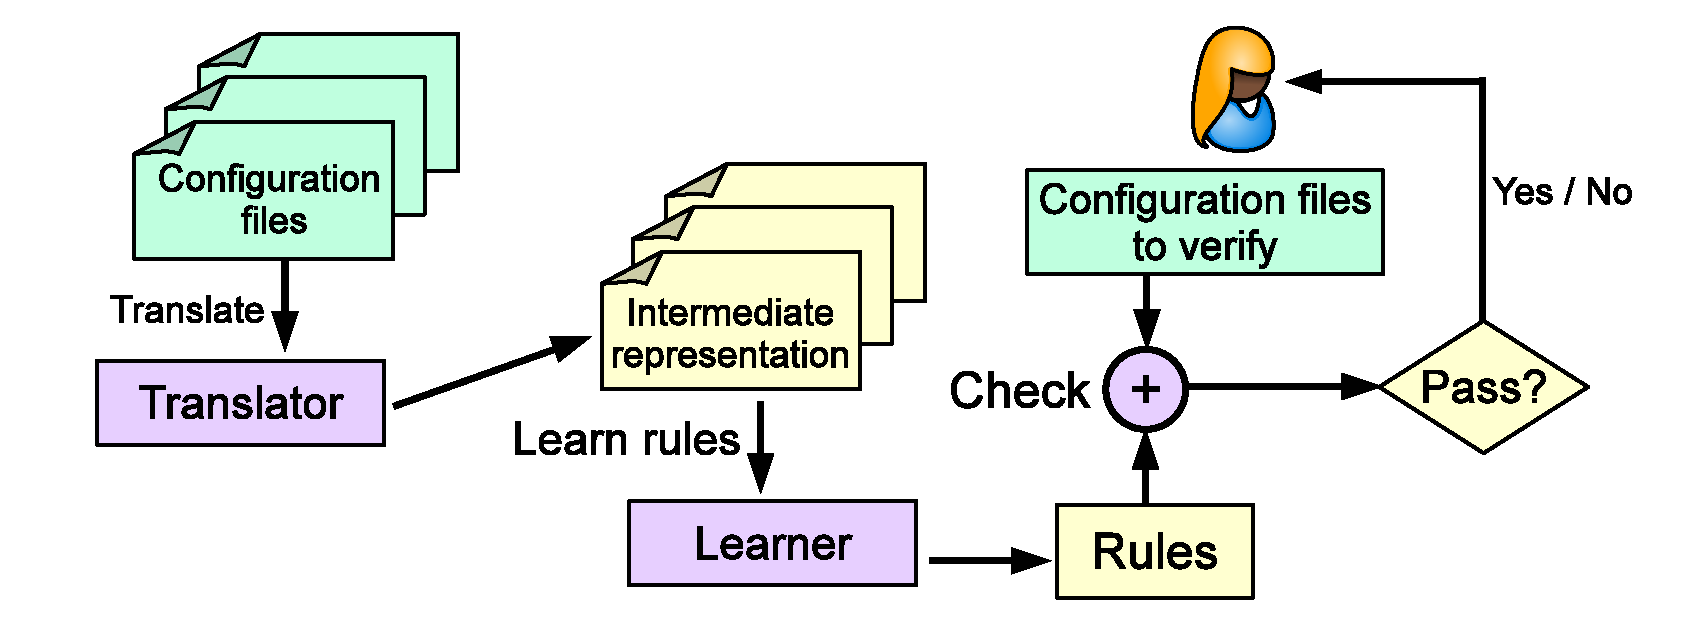
\includegraphics[width=0.78\textwidth]{figs/overview}
\caption{An overview of the \app system architecture}
\label{fig-overview}
\end{figure}




A rule R is added to the set of all rules,
  if $\exists$ learning file f s.t. R(f) is non vacuously true
That rule R is then removed from the set of all rules,
  if $\exists$ learning file f st R(f) is false.

This is accomplished in two passes.
First we collect all possible rules for every file.
Then we merge the all the rules to create our final set.
This conviently gives rise to an embarresingly parallel situation, which Haskell allows us to easily take advantage of by
  using the parallel mapping library parmap.

\begin{lstlisting}
  potentialRules = parmap findAllRules learningSet.
  finalRules = foldl1 mergeRules potenialRules
\begin{lstlisting}


Each rule is of the Attribute typeclass, which means a rule must support the following operations:
\begin{lstlisting}
class Attribute r where
  learn :: ConfigFile Common -> [r]
  merge :: [r] -> [r] -> [r] 
  check :: [r] -> ConfigFile Common -> Error
\end{lstlisting} 


\section{Ordering}
\subsection{learn}
  For a single given file, we take very line ordering to be a rule.
\subsection{merge}
  Then when merging these sets of rules, we take the intersection of the rules infered on the individual files.
  Maybe we could also do something like only taking rules that show up multiple times.
\subsection{check}
  To check a file by using a rule set, we simply take all the rules that are releveant to the user's file.
  Rules that are relavent are the ones where both parts of the ordering are present.
  We learn the rule set for the user file, and every rule in the learned set must be present in the user file.
 

\section{Translator}
\label{sec-trans}

The translator takes as input a sample dataset of configuration files and transforms it into another set of files written in
typed and well-structured representations.
The translator can be seen a parser, and it is only
used to generate an intermediate representation for post-processing, 
such as learning rules (see $\S$\ref{sec-learn}).
Coupled with rules generated by learner module,
we will have a complete language model to verify configuration files
of our interest.

Translating or parsing is system dependent. In other words, for MySQL
and HDFS, we need to develop different parsers to handle each of them,
respectively. \app allows users to 
provide extra help to the translator
for their specific system configurations,
but it is not required.

The majority of entries in a configuration files are assignments. Our first attempt was to simply
translate every key-value entry {\tt {k = v}} into a triple $(k, v, \tau)$, where $\tau$ is a type of 
$v$. However, sometimes we could not fully determine the type of key 
based on a single example value. For this reason, we introduced {\emph {probabilistic types}}.

Consider the following example.

\noindent{\tt {foo = 300}}\\
{\tt {bar = 300.txt}}

Most likely {\tt foo} should be an integer, but it could also be a string.
In the second case, we can learn the rule stating 
$ \texttt{foo} \in \textsf{substrings}(\texttt{bar})$. 
Instead of assigning one type to a value, the translator assigns a distribution of types 
to a value, an idea closely related to existentially quantified 
types~\cite{Launchbury93lazyfunctional}. 

Formally, we define probabilistic types as follows: let $\mathcal{T}$ be a set of basic types (cf. Table~\ref{table:kysymys}).
A probabilistic type built from $\mathcal{T}$ is a list of pairs 
$[(\tau_1, p_1),\ldots,(\tau_n, p_n)]$,
such that $\tau_i \in \mathcal{T}$, $0 \le p_i \le 1$ 
and $\Sigma p_i = 1$. 
These probabilities are updated each time a new example value 
for a key is encountered.

When a value has a probabilistic type, we generate rules for all its types.
This means that by assigning {\texttt{foo}} a probabilistic type 
(\eg, {\tt (\texttt{foo}, 300, [(\textsl{Int},90\%), 
(\textsl{String},10\%)])},
we would generate rules for both strings and integers.
Once the type inference can uniquely determine the type, 
the probability of all other types is set to zero, 
and the associated rules are withdrawn.

In \app, the set $\mathcal{T}$ contains strings, integers, file paths, 
sizes, and IP addresses. With every type, we associate a list of templates 
that are used to learn the rules about those files. Table~\ref{table:kysymys} contains
the most important types and templates.

\begin{table}
\caption{Table of types, along with associated templates, used in \app}
  \begin{tabular}{| l |  l |}
    \hline
    Type &  Template \\ \hline
    Integer & $X = Y, X\neq Y, X \leq Y, X < Y, X * Y < Z, \ldots $\\ \hline
    String & $\textsf{substr}(U, V), \textsf{prefix}(U,V), \textsf{suffix}(U,V), \ldots$   \\ \hline
    File Path & $\textsf{isFile}(F), \textsf{isDir}(D),\ldots$   \\ \hline
    Size & Similar to integers   \\ \hline
    Port & $P_1 > P_2$ \\ \hline
    IP Addr.  & $\textsf{sameSubnet}(addr1, addr2)$   \\
    
    \hline
  \end{tabular}
\label{table:kysymys}
\end{table}


In general, the templates works as follows: if there are two entries ${\tt {k1 = v1}}$ and 
${\tt {k2 = v2}}$, let $t(X, Y)$ be a template that can be applied to those values (w.r.t. their types).
If $t(v1, v2)$ holds, \ie, the template condition is valid for those concrete values, then we will add a rule
$t(k1, k2)$ to a list of potentially correct specifications. Note that the rule expresses a relation between variables.

With the help of probabilistic types, we addressed ambiguities during the parsing phase. Another problem that we need to solve
is that configuration files sometimes contain a simple version of the {\tt {if-then}}, such as in Apache HTTPD, that 
sets conditions for which an action should be applied. Therefore, we also add this guard to our entry 
during the parsing phase. We first check if the guard is true before deriving a rule; otherwise, we skip the entry.

To summarize, the translator translates every entity ${\tt {k = v}}$ in a configuration file into a quadruple entry
$$(g,k,v,\textsf{List}[p_1:\tau_1, \ldots, p_n:\tau_n])$$

For an entry, we denote the corresponding guard by $g(e)$, the key by $k(e)$, the value by $v(e)$, and the probabilistic
type list by $typelist(e)$. 

\com{Note that typing is also a system module than 
can be easily extended to support more types. 
In that case the user will need to provide rules for type inference 
and probability distributions for values where type inference is ambiguous.
}


\section{Learner}
\label{sec-learn}

The goal of the learner module is to derive rules and constraints from
the intermediate representation generated by the translator.
It has two components.
The first component ($\S$\ref{subsec-rules}) 
learns rules for checking misconfiguration errors like
missing entry, ordering, and fine-grained value correlation errors. 
These errors tend to cause total system failures.
%Once the configuration file has been validated against such rules, 
%the user may choose to invoke a more sensitive constraint checker. 
The second component ($\S$\ref{subsec-constraints}) 
aims to derive 
constraints on entries to check for suspicious (or anomalous) values 
that may violate standard practice. These anomalies can cause partial 
degradation of the system, such as significant reduction in performance, or even 
total failure as in Example~4 of $\S$\ref{sec-motiv}.

\subsection{Derivation of Probabilistic Rules}
\label{subsec-rules}

The first component learns rules that must hold over 
multiple parts of a configuration file.

\para{A strawman solution.}
We now first present a strawman solution (employed by
previous work~\cite{santolucitoCAV, zhang14encore}) that uses 
a set of correct configuration files as a learning set, 
from which it is possible to derive rules 
that must hold with absolute certainty. 
In practice, however, it is difficult to obtain a set of files 
that is both guaranteed to be without misconfiguration 
and large enough to learn many rules of configuration files.
This usually requires manual verification of the learning set, 
which is prone to error.

As a result of this restriction, 
these efforts only consider a rule if it holds over exactly every file in 
the learning set. This behavior can be formally described as follows:

\begin{small}
\begin{flalign*}
C =&\ \text{Correct Learning Set}\\
\text{::}\ & \text{\{Configuration Files in Intermediate Representation\}}\\
LR =&\ \text{Learned Rules :: \{Rule\}}\\
RR =&\ \text{Reported Rules :: \{Rule\}}\\ 
LR =&\ \{ r\ \mid \forall file \in C,\ holds(r,file)\} \\
RR =&\ \{ r\ \mid r \in L\ \land \neg\ holds(r,userfile) \}
\end{flalign*}
\end{small}

Each rule can be thought of as a mapping from 
lines $j$ and $k$ in a configuration file to a relation, $R$.

\[
\{ Rule = (a_j, a_k) | j \neq k \} \rightarrow \{ R \}
\]

Specifically, $a_j$ and $a_k$ are two different lines from our
intermediate representation, or more formally, $j \neq k \land
a_j, a_k \in \{ L \}$ where is the set of lines (key-value pairs) found
in the learning set. The relation $R$
is a Boolean function specific to the error to detect. 
As an example, to detect the error that key $k_1$ must always 
have a value greater than key $k_2$, the relation $R$ is $>$.

\para{Our approach.}
In \app's leaner module, the rule learning mechanism is tolerant 
enough to accept a dataset {\em full of} incorrect configuration files.
Rather than manually correcting each file, 
we extend the previous formalism to run probabilistic learning
on our intermediate representations (generated by the translator). 

Our probabilistic approaches for learning the entry missing, 
ordering, and fine-grained value correlation rules stem 
from existing work with building 
the non-probabilistic versions of these rule-learning algorithms. 
We start with the idea that for each of these rules, 
we are going to consider all possible pairs of keys that appear in every 
file, and for our learning process, calculate the likelihood that each of 
these pairs constitute a rule. 
In essence, this is a mechanism that will consider many different possible 
pairs of lines of entries in the file, 
and attempt to compile a set of these pairs 
that are expressed more often than others as a basis for finding patterns 
within the example set that can be used to evaluate new files.

More formally, this approach can be defined as follows. 
The output of our learning algorithm is augmented to a map from 
key-value pairs to a probability distribution over number of possible 
relations.

\[
\{ P\_Rule = (a_j, a_k) | j \neq k \} \rightarrow \{ (R_1, R_2, ... , R_n) \}
\]

We can think of each of these $(a_j, a_k)$ as possibly having a different relationship, defined by the set $\{ R_i \}$, which cover the entire outcome space of possible relationships between the two values $(a_j, a_k)$.

For the entry missing rules, we define $R_1$ as the event that $a_j$ and
$a_k$ appear together, and $R_2$ to be the event that $a_j$ appears
without $a_k$, or by the transitive equivalent, $a_k$ appears without
$a_j$. For the ordering rules, we define $R_1$ as the event that
$a_j$ appears before $a_k$ and $R_2$ be the event that $a_k$ appears
before $a_j$. For the value correlation rules, we define $R_1$ as the
event that $a_j \leq a_k$, $R_2$ the event that $a_j = a_k$, and $R_3$
the case that $a_j \geq a_k$. Notice that the $R_i$ do not have to be
disjoint, but only have to union to the entire probability space.

By examining the learning set, we will derive a distribution of the set $\{R_i\}$ based on how many times we observe an occurrence of each relation. This distribution will then be used at checking time to determine if a user's configuration has broken a likely rule. 

\begin{small}
\begin{flalign*}
I\ \ =&\ \text{Incorrect Learning Set}\\
\text{::}\ & \text{\{Configuration Files in Intermediate Representation\}}\\
LP =&\ \text{Learned Probabilistic Rules :: \{(P\_Rule)\}}\\
RP =&\ \text{Reported Probabilistic Rules :: \{(P\_Rule)\}}\\
LP =&\ \text{count\_relation\_occurrences}(I)\\
RP =&\ \{ r\ \mid r \in LP\ \land \Pi(r)>p \land \neg r(userfile) \}
\end{flalign*}
\end{small}

A rule will be reported as broken if the probability the rule is correct, $\Pi$, is greater than some user defined constant, $p$. This constant can be adjust to the user's preference. A small $p$ will increase the likelihood of finding an error, but also increase the number of false positives that are reported.


\subsection{Learning Suspicious Constraints}
\label{subsec-constraints}

With a configuration file that has been verified against catastrophic
failures (\eg, entry missing, type and ordering errors), 
the user may also want to find out more subtle issues.
Anomalous values can cause tricky, but impactful, performance and memory
issues that are hard to debug, as discussed in Example 4 of 
$\S$\ref{sec-motiv}. 
Consequently, anomalous values should be flagged and a warning returned
to the user indicating the violation.

We now describe the technique we use to detect anomalous values for 
numerical attributes. Let $A$ be the set of attributes contained in the 
configuration files in the sample dataset. 
Let $A_n$ be the subset of attributes of $A$ which are numerically typed. 
Then, for each attribute $a \in A_n$, we construct a vector $v_a$ of the 
values corresponding to attribute $a$, seen over the entire sample dataset.
For each $v_a$, we compute 
an interval  $$[\hat{v_a} - 50*MAD(v_a), \hat{v_a} + 50*MAD(v_a)],$$ 
where $\hat{v_a}$ represents the median over the values 
in $v_a$ and $MAD(v_a$) refers to the 
median absolute deviation. 
This is a variant of a standard outlier detection test, namely the Hampel identifier.\footnote{Mathematically, $MAD(v_a) = 1.4826* median(|v_a - \hat{v_a}|)$, estimating standard deviation 
for a normal distribution.} 
In the checking phase, as long as the checker finds a value for a numerical 
attribute in the checked file outside of this interval, 
a warning would be printed to the user indicating the violating value, 
the attribute, and the upper or lower Hampel threshold. 

The intuition behind this is that if the user has input a value 
that falls outside of an interval containing values that are considered 
``normal'' over the entire sample dataset, 
that value will probably cause an error, in particular for performance. 
We cannot know for sure if this value will cause an issue. 
For instance, a user might have a machine with 
particularly high-end hardware, 
in which case a value beyond the upper Hampel threshold may be appropriate. 
 %rule interface, psudocode of algorithm, association rule learning, details on each module 
% Graph Analysis
% Rahul

\iffalse

# Structure and Core Points]
#
# @author rahuldhodapkar
#
#   Below is a structured summary from which I tried to write my section.
#   I have tried to include points of emphasis and a general argumentative
#   flow from which to work.
#
#   This should be used as a rubric to determine if we have hit all of
#   the critical beats of this section, or if there are core points
#   still missing.
#

[Problem Definition]

    - What is the intermediate representation from the learner?
        -> why can / should we interpret it as a graph?
        -> what benefits does this give over neural-networks?

    - What is the problem faced by the verification field?
        -> how can we be more intelligent about detecting false-positives?
        -> introduce the degree metric concept.

    - What are some problems outside the verification field that this can
      help answer?
        -> Introduce the idea of algorithmic complexity.
        -> We introduce a heuristic to measure the complexity of configuration
           files, drawn from information in the rule graph.

[The degree metric]

    - Definition of the degree metric.
        -> Sub-definition of edge slice sets.
        -> Sub-definition of edge set size => |*| operator

    - How will the degree metric be used to prune false-positive rules?
        -> specific definition of the weighting procedure.

[A heuristic for complexity of configuration files]

    - Definition of the complexity heuristic.

    - Example of the complexity heuristic on a graph (? space permitting)

    - Additional interpretations of the Rule Graph

\fi

\section{Rule Graph Analysis}
\label{sec-post}

The learner outputs a set of rules learned from the training set as
described in Sec.~\ref{sec-learn}. Recall that a rule is 
an implication relationship of the form $r = S \implies p(S,T)$.
This data is necessary to perform the core verification task,
but can also be used for further analysis. By interpreting the rules as a graph (which
we call the \textit{Rule Graph}), we can 
use tools from graph theory to extract information
about the configuration space that can improve the quality of the learned model.
We inspect properties of this 
Rule Graph to sort reported errors by those most likely to be valid.
To demonstrate the additional value of the Rule Graph, we
also use it to estimate the complexity of a configuration file.

Accessibility of the Rule Graph is a useful property of the association 
rule learning technique applied by \app.
While it is possible to analyze the models from other machine learning techniques, such as neural networks~\cite{lei2016rationalizing} and
conditional random fields~\cite{raychev2015predicting}, these analyses require a deep knowledge of the applied techniques.
In contrast the Rule Graph is a relatively simple, yet information rich, representation of the learned model.
The following section provides a precise definition of the Rule Graph
and demonstrates useful metrics we derive for the purposes of ranking reported errors
and complexity analysis.

\subsection{Rule Ordering}
\label{sec:ruleorder}

We define the \textit{Rule Graph} as a directed hypergraph $H = (V,E)$,
   with vertices $V = \{ keywords \}$ and labeled, weighted edges $E = \{ (V_s, V_t, l, w) \}$.
The set of edges is constructed from the learned rules, using the source and target keyword sets as sources and targets respectively, the predicates as labels, and the confidence as weights:
%
\begin{align*}
\forall r \in & Learn(\trainingSet).\ \exists e\ \in E.\\
              & V_s = S_r \land V_t=T_r \land l=p_r \land w =
\textit{confidence(r)}
\end{align*}

We will also denote $E_{V_1, V_2} \subset E$ as the \textit{slice set} 
of $E$ over $V_1, V_2$.
We can think of $E_{V_1, V_2}$ as being the subset of edges in $E$ 
such that each source set $V_s$ shares a vertex with $V_1$
and each target set $V_t$ shares a vertex with $V_2$.
Formally: 

\begin{align*}
    E_{V_1, V_2} = \{ \left( V_s, V_t, l, w \right) \in E \ \mid \ & \exists v_1 \in V_1 \land v_1 \in V_s \ \land\\
    & \exists v_2 \in V_2 \land v_2 \in V_t \}
\end{align*}


We denote a standalone vertex $v$ in our subscripts as notational 
convenience for the singleton set containing that vertex $v$.

The size of an edge set is the sum of all weights in that set, so:

    $$|E| = \sum_{(S, T, l, w) \in E} w$$

The use of the support and confidence thresholds $t_s$ and $t_c$ in the learner ensure 
that all weights in the Rule Graph are positive.

We define a measure of degree $\mathcal{D}(v)$ for each vertex $v$ as the sum of 
in-degree and out-degree. Explicitly, for a vertex $x \in V$:

    $$\mathcal{D}(x) = \sum_{v \in V} |E_{x, v}| + \sum_{v \in V} |E_{v, x}|$$

We may now use this measure to rank our errors.
The more rules of high confidence are extracted for a keyword by the learner, 
the higher the $\mathcal{D}(v)$ of the corresponding vertex in the Rule Graph.
In our final analysis, we use this classification to
order the reported {\it errors} by estimated importance.

Keywords (specifically their corresponding vertices)
of low $\mathcal{D}(v)$ may be rarer configuration
parameters where rules learned are more likely to be governed by 
tehchnical necessity, rather than industry convention. As such, errors
reported involving low-degree keywords are more likely to be errors
of high significance and should be presented with high importance
to users of \app.

Specifically, for an error reported by \app on a rule $r$ involving
keywords $K$, we rank the errors by:

    $$\textit{RANK(r)} = \frac{\sum_{k \in K} \mathcal{D}(k)}{|K|}$$

The results from ranking errors in this way are presented later in
the paper.

\subsection{Complexity Measure}

We may also use the Rule Graph to advance our general knowledge
of the configuration space, outside the strict confines of a
verification system. As an example, we present a heuristic
for configuration file complexity based on the topology of the
Rule Graph. This measure of complexity could be used by software
organizations to manage configuration files in much the same way
as Kolomogrov complexity~\cite{kolmogorov1965} is used to manage code - identifying
potentially brittle configurations for targeted refactoring.

For a configuration file with a set of keywords $K$
and a Rule Graph $H = (V, E)$, we define our complexity measure:

\begin{equation}
    \mathcal{C}(K, H) = \sum_{k \in K} \
        \begin{cases}
            1 * (1 - \frac{|E_{k, K}|}{|E_{k, V}|}) & \text{if}\ \ |E_{k, V}| > 0 \\
            1 & \text{otherwise}
        \end{cases}
\end{equation}

The complexity measure, $\mathcal{C}$, can be thought of as an
extension of the na\"ive line-counting measure of complexity.
When a keyword in the configuration file is present in the Rule Graph,
we may consider the set $E_{k, K}$ to be all learned rules involving
keyword $k$ that
are {\it relevant} to the configuration file being examined. 
The set $E_{k, V}$ denotes {\it all} learned rules involving $k$.
Given these sets, we may think of $\frac{|E_{k, K}|}{|E_{k, V}|}$
as representing the amount that $k$ is constrained in the current
configuration file relative to how much it could be constrained
in the global configuration space. The more constrained a configuration
keyword in a particular configuration file, the {\it less} it should
contribute to the complexity (hence $1 * (1 - \frac{|E_{k, K}|}{|E_{k, V}|})$).
If a keyword is not constrained at all in the current configuration
file or is not present in the Rule Graph, we revert to the standard
counting metric of complexity. 

While an in-depth evaluation of the complexity metric presented here
is out of scope for this paper, we use this measure to
demonstrate the flexibility of the rule graph, and potential
for further applications.



\section{Implementation and Evaluation}
\label{sec:eval}

We have implemented a tool, \app, and evaluated it based on real-world configuration files taken from Github.
\app is written in Haskell and is available open source at \textit{url redacted for anonymity}.
Thanks to the Haskell's powerful type system, the implementation can easily be extended with new rule classes or applied to different configuration languages with minimal change to the rest of the code base.
A user only needs to provide the functions for the rule interface (a typeclass in Haskell) to 1) learn relations from a single file 2) merge two sets of rules and 3) check a file given some set of rules.

\subsection{Evaluation}

To evaluate our \app prototype, we require a separate training set and test set. 
For our training set, \trainingSet, we use a preexisting set of 256 
industrial MySQL configuration files collected in previous configuration 
analysis work~\cite{configdataset}.
This is an unlabeled training set, though most of the files have some errors.
For our test set, we collected 1000 MySQL configuration files 
from Github, and filtered the incorrectly formatted files out for a final 
total of 973 files.
In our evaluation, we focus on MySQL for comparability of results, but \app can handle any configuration language (that can be parsed to the intermediate representation from Sec.~\ref{sec:trans}).

We report the number of rules learned from the training set and the number of errors detected in the test set in Table~\ref{table:learning}.
One interesting note is that without probabilistic types we learned 327 fine grained rules and detected 1367 errors.
By introducing probabilistic types, we remove 114 incorrect rules and thereby remove 1023 false positives.
We are guaranteed these are all false positives since there cannot be a correct rule of relating the types $size*size$ and $size$ because of the semantic interpretation of the $size$ units.

We also provide the support and confidence thresholds, $t_s, t_c$, used in this evaluation.
These number can be adjusted by the user as a slider to control the level of assurance that their file is correct.
Since these settings depend on both the user preference and training set quality, we simply choose values for which \app reports reasonably sized output.
This is a determined by the user by examining the rule set output over the training set.
Following common practice from association rule learning, initial values for support are confidence are generally 10\% and 90\% respectively.

We record the histogram of errors across the test set in Figure~\ref{fig:histo}.
This is intuitively an expected result from randomly sampling Github - most repositories will have few errors, with an increasingly small number of repositories having many errors.

\begin{figure}[h]
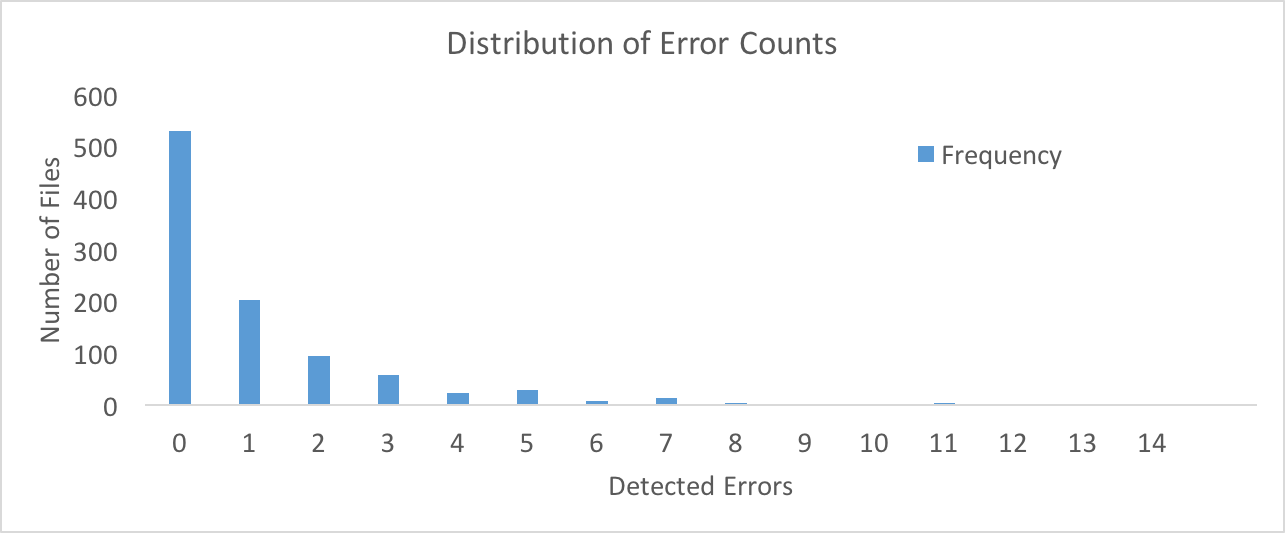
\includegraphics[width=\textwidth]{figs/histogram.png}
\caption{Histogram of errors - 14 errors were detected in 1 file}
\label{fig:histo}
\end{figure}

\begin{table}[h]
\centering
\caption{Results of \app}
\label{table:learning}
\setlength{\tabcolsep}{0.5em}
\begin{tabular}{|c|c|c|c|c|}
\hline
{\bf Class of Error } & {\bf \# Rules Learned} & {\bf \# Errors Detected} & {\bf Support} & {\bf Confidence}\\ 
\hline
\hline
Order        & 13  & 62   & 6 \%  & 94 \% \\ 
Missing      & 53  & 55   & 2 \%  & 71\% \\ 
Type         & 92  & 389  & 12 \% & 70\%  \\ 
Fine-Grain   & 213 & 324  & 24 \% & 91\%  \\ 
Coarse-Grain & 97  & 237  & 10 \% & 96\% \\ 
\hline 
\end{tabular}
\end{table}

The errors reported may have varying impacts on the system, ranging from failing to start, runtime crash, or performance degradation.
However, since \app is a probabilistic system, it is also possible that some errors are false positives, a violation of the rule has no effect on the system.
Note that in contrast to program verification, we do not have an oracle for determining if a reported error is a true error or a false positive.
While we can run a program to determine the effect a specification has on the success of compiling/running the program, no such test exists for configuration files.
Because configurations are dependent on the rest of the system (\ie, the available hardware, the network speed, and the usage patterns), we cannot simulate the all conditions to determine if a reported error will cause system failure.
As evidenced by Example~\ref{ex:fine}, some misconfigurations will only cause greater than expected performance degradation, and only under particular traffic loads.
In light of this, the definition of a true error is necessarily imprecise.

Although we cannot identify false positives, we can identify true positives by examining online forums, like StackOverflow.
On these forums we find reports that particular configuration settings have caused problems on real-world systems.
Furthermore, any error for which we can find evidence online is likely to be more problematic than errors that do not have an online record, 
  using the reasoning that this error has caused enough problems for people to seek help online.
In this case, we would like \app to sort the errors by their importance or potential severity.
To achieve this sorting we use the rule graph analysis metric described in Sec.~\ref{sec:ruleorder}.

To estimate the impact of this metric, we track the rank of known true positives with, and without, the augmented rule ordering in Table~\ref{table-casestudy}.
For this table, we picked the known true positive rules, listed in the Errors column, and pick configuration files in the test set that have these errors.
We picked 3 files for each true positive by choosing the files with the highest number of total reported errors in order to clearly observe the effects of our optimizations.
Although this gives a more clear picture of the effect of our optimizations, it results in a slightly inflated false positive rate.

We test the following conditions; just rule graph analysis (RG) to sort the errors, just probabilistic types to filter the rules (PT), and both optimizations at the same time (RG $\land$ PT).
For each entry we list X/Y, where X is the rank of the known true positive, and Y is the total number of errors found in that file.


\newcommand{\tablewidth}{6cm}
\definecolor{Gray}{gray}{0.80}
\newcolumntype{g}{>{\columncolor{Gray}}c}


\begin{table*}[tbp]
\centering
\caption{Sampled misconfiguration files for error detection evaluation.}
\label{table-casestudy}
\setlength{\tabcolsep}{0.5em}
\begin{footnotesize}
\begin{tabular}{|c|c|c|g|g|c|}
\hline
{\bf Errors} & {\bf URLs} & {\bf None} & {\bf PA} & {\bf PT} & {\bf PT$\land$ PA}\\ 
\hline
\hline
\multirow{3}{*}{\parbox{\tablewidth} {\scriptsize ORDERING ERROR: Expected ``innodb\_data\_home\_dir'' BEFORE ``innodb\_data\_file\_path''} }
& url & 12/12 & 3/12 & 5/5 & 3/5 \\
& url & 11/11 & 2/11 & 3/3 & 3/3 \\ 
& url & 9/9   & 3/9  & 4/4 & 3/4 \\ 
\hline

\multirow{3}{*}{\parbox{\tablewidth} {\scriptsize MISSING ERROR: Expected ``key\_buffer'' WITH [isamchk]} }
& url & 6/10 & 2/10 & 2/4 & 2/4 \\ 
& url & 2/3 & 3/3 & 2/3 & 3/3 \\
& url & 2/3 & 3/3 & 2/2 & 3/3 \\  
\hline

\multirow{3}{*}{\parbox{\tablewidth} {\scriptsize TYPE ERROR: Expected an integer for “slow\_query\_log”}}
& url & 32/34 & 1/34 & 5/7   & 1/7 \\ 
& url & 9/20  & 2/20 & 10/11 & 2/11 \\  
& url & 9/19  & 2/19 & 10/11 & 2/11 \\
\hline

\multirow{3}{*}{\parbox{\tablewidth} {\scriptsize FINE GRAINED ERROR: Expected \\ ``max\_connections'' * ``sort\_buffer\_size'' $\geq$ ``key\_buffer\_size''}}
& url & 30/34 & 18/24 & 6/7 & 3/7 \\ 
& url & 23/25 & 9/25  & 8/9 & 3/9 \\  
& url & 20/23 & 14/23 & 6/7 & 5/7 \\
\hline

\multirow{3}{*}{\parbox{\tablewidth} {\scriptsize INTEGER CORRELATION ERROR: Expected ``max\_allowed\_packet'' $<$ ``innodb\_buffer\_pool\_size''} }
& url & 29/32 & 8/32 & 11/14 & 4/14 \\ 
& url & 22/23 & 2/23 & 9/10  & 2/10 \\  
& url & 10/12 & 4/12 & 4/4   & 2/4 \\
\hline

\end{tabular}
\end{footnotesize}
\end{table*}




\subsection{False Positive Rate}

Because \app detects complex and subtle misconfigurations that, for example, may cause performance degradation in a high traffic load, false positives are system and use-case dependent and therefore ill-defined.
However, we report an estimation of the false positive rate for comparison to other tools.
To estimate a false positive rate, we asked two industry experts, one from MongoDB and one from Microsoft, to independently classify all errors from Table~\ref{table-casestudy}.
For each unique error reported in Table~\ref{table-casestudy} (a total of 70 unique errors), the expert was asked to classify the error as: definitely false positive, potential true positive, or definitely true positive. 
The MongoDB expert rated 13/70 errors as definitely false positives. 
The Microsoft expert rated 8/70 errors as definitely false positives. 
The similarity between experts is suggestive that these are approximately correct classifications.

The resulting false positive rate is then estimated to be 11\%-18\%.
This is in the range of existing work, for example in the EnCore tool, which had a false positive rate of 13\%,21\%,32\% for MySQL, Apache, and PHP respectively~\cite{encore}.
We note again that as opposed to a tool like EnCore, which is used mainly to detect initialization errors, thanks to the complex relations that can be learned, \app also learns misconfigurations causing runtime performance degradation.
This means \app generates a larger rule set, and false positives cannot be guaranteed, \ie there may be some environment conditions that will cause a ``false'' positive to become a true positive.

In contrast, a true positive can be confirmed as such based on evidence of unwanted system behavior.
The errors listed in Table~\ref{table-casestudy} are confirmed true positives, evidenced by posts on help forums.
\app detected and reports these errors in the 15 code repositories listed in the URL column of Table~\ref{table-casestudy}. 
These are real-world configuration files that contain errors that may be unknown to the maintainers of the repositories.
%The errors were not submitted as patches to the repository owners, since it is possible the owner of the repository has a user case for this configuration file that will not trigger the unwanted behavior.

\subsection{Runtime Performance}
We also evaluate the speed of \app.
Generally, once a set of rules has been learned, it is not necessary to rerun the learner.
However, we have only used \app to build rules for MySQL, but any configuration language can be analyzed with \app given a training set, which requires rerunning the learner.
Additionally, in an industrial setting, the available training set may be much larger than ours, so is important that the learning process scales.
We see in Table~\ref{table:training} that \app scales roughly linearly.

We compare \app to prior work in configuration verification, ConfigC~\cite{santolucitoCAV}.
ConfigC scales exponentially because the learning algorithm assumes a completely correct training set, and learns every derivable relation.
With \app, we instead only process rules that meet the required support and confidence, reducing the cost of resolving to a consistent set of rules. 
The times reported in Table~\ref{table:training} were run on four cores of a Kaby Lake Intel Core i7-7500U CPU @ 2.70GHz on 16GB RAM and Fedora 25.

\begin{table}[h!]
\centering
\caption{Time for training over various training set sizes}
\label{table:training}
\setlength{\tabcolsep}{1em}
\begin{tabular}{|c|c|c|}
\hline
{\bf \# of Files for Training} & {\bf ConfigC (sec)} & {\bf \app (sec)}\\ 
\hline
\hline
0    & 0.051    & 0.051  \\ \hline
50   & 1.815    & 1.638  \\ \hline
100  & 13.331   & 4.119  \\ \hline
150  & 95.547   & 10.232  \\ \hline
200  & 192.882  & 12.271  \\ \hline
256  & 766.904  & 15.627  \\ 
\hline
\end{tabular}
\end{table}


%
\section{Discussion and Limitations}

This section discusses a few \app's limitations
and possible solutions.

\para{Legal misconfigurations.}
While \app can check for diverse configuration errors without
human intervention, most of the existing proactive 
misconfiguration detection techniques,
including \app, cannot handle configuration errors
resulting from events occurred during the system runtime.
Such configuration errors are referred to as {\em legal misconfigurations}%
~\cite{yin11anempirical}. In particular, 
many parameter misconfigurations have 
perfectly legal types and values, 
but do not deliver the functionality intended by users. 
For example, after a website's traffic significantly increases,
the parameter {\tt Max\_key\_buffer} in MySQL may not 
be able to handle increasingly more data traffic,
thus leading to the outage of the whole system.
These cases are more difficult to detect by
automatic checkers and may require more user training or
better configuration design.
A potential solution is to combine existing misconfiguration diagnosis
tools, \eg, X-ray~\cite{attariyan12x-ray} 
and ConfAid~\cite{attariyan10automating},
with \app in order to enhance the 
misconfiguration checking capability.

\para{Misconfiguration across software components.}
As exposed by Yin {\em et al.}~\cite{yin11anempirical},
cross-software configuration correlation problems also account
for a considerable number of misconfiguration cases.
For example, in a LAMP-based Web server, one entry in 
PHP configuration file, {\tt mysql.max\_persistent = 400}
may make users encounter a ``too many connections'' error,
because a correlated entry in the underlying MySQL's configuration
file assigns {\tt max\_connection} to 300, which is less
than the MySQL connection numbers in PHP's configuration file (\ie, 400).
It is quite difficult to detect such a type of tricky error
through leaning approaches, because not only users or engineers 
are not aware of the hidden interactions~\cite{xu15systems},
but also it is hard to obtain a global knowledge to the entire
configurations due to the business privacy concerns of
each software provider.
One possible solution to this problem might be to introduce
some cryptographic protocol, \eg, private set
intersection~\cite{kissner05privacy}, to privately extract the
overlapping entries, \eg, {\tt mysql.max\_connection} in the 
above MySQL and PHP case, for double-checking.

\para{Network configuration verification.}
\app mainly focuses on software configurations, \eg, MySQL and Apache,
so that our approach is limited to support network configuration
verification. This is because network configurations have quite
different representations, format and rules from software configurations,
since network configurations are typically written in 
more domain-specific policy languages.
In fact, many network verification tools, 
\eg, NoD~\cite{lopes15checking} and 
Dobrescu {\em et al.}~\cite{dobrescu14software},
have been proposed to check whether network configurations
meet their specifications.

\para{More complex configuration structure.}
The current \app mainly targets key-value configuration files,
but in practice many systems, \eg, OpenStack~\cite{OpenStack},
employ very complex configuration format and structure,
which \app cannot handle.
Verifying such structurally complex configurations typically needs
\app to learn a much more sophisticated language model,
which is challenging in practice.
Recent efforts~\cite{raychev15predicting, raychev16learning} 
may present a possible solution on this limitation.
These techniques can learn a call-graph from a training program set,
and check a new program based on properties extracted from this
generated call-graph. If we look a structurally complex configuration 
file as a program in these tools, we may be able to use a similar way
to verify whether the configuration file violates any 
property of our interest. 
 %TODO merge with related

\section{Related Work}

\iffalse
Configuration verification has been considered a promising way  
to tackle misconfiguration problems~\cite{xu15systems}.
Nevertheless, a practical and automatic configuration
verification approach still remains an open problem.

\para{Language-support misconfiguration checking}
There have been several language-support efforts proposed for preventing
configuration errors introduced by fundamental deficiencies in
either untyped or low-level languages. For example, in the network
configuration management area, administrators often
produce configuration errors in their routing configuration files.
PRESTO~\cite{enck07configuration} 
automates the generation of device-native configurations
with configlets in a template language. 
Loo {\em et al.}~\cite{loo05declarative} adopt Datalog to reason about 
routing protocols in a declarative fashion. 
COOLAID~\cite{chen10declarative} constructs
a language to describe domain knowledge about devices and
services for convenient network reasoning and management.
Compared with the above efforts, our work focuses on software systems, 
\eg, MySQL and Apache, and our main purpose is to automate configuration
verification rather than proposing new languages 
to convenient configuration-file writing. 

\para{Misconfiguration detection}
Misconfiguration detection techniques aim at checking configuration
efforts before system outages occur.
Most existing detection approaches check 
the configuration files against a set of predefined correctness 
rules, named constraints, and then report errors if 
the checked configuration files do not satisfy these rules.
Huang {\em et al.}~\cite{huang15confvalley},
for example, proposed a 
language, ConfValley, to validate 
whether given configuration files meet administrators' specifications. 
As opposed to our work, ConfValley does not
have inherent misconfiguration checking capability, since it only offers
a language representation and requires administrators to
manually write specifications, which is an error-prone
process. On the contrary, our work does not need users to manually
write anything.

Several machine learning-based misconfiguration detection efforts 
also have been proposed~\cite{yuan11context, zhang14encore, xu16early}.
EnCore~\cite{zhang14encore} introduces a template-based
learning approach to improve the accuracy of their learning results.
The learning process is guided by a set of predefined rule templates
that enforce learning to focus on patterns of interest.
In this way, EnCore filters out irrelevant information and reduces
false positives; moreover, the templates are able to express
system environment information that other machine learning
techniques cannot handle.
Compared with EnCore, \app has the following advantages.
First, \app does not rely on any template. 
Second, EnCore cannot detect missing entry errors, type errors,
ordering errors and fine-grained integer correlation errors,
but \app can detect all of them.
Finally, \app is a very automatic system, but
EnCore needs significant human interventions, \eg, system parameters
and templates.

PCheck~\cite{xu16early} aims to add configuration checking code to the system source code by emulating potential commands and behaviors of the system. 
This emulation is a ``white-box'' approach and requires access to the system's source code.
One drawback to this approach is that for some systems (\eg, ZooKeeper) whose behavior is 
hard to emulate, PCheck cannot automatically generate the corresponding checking code.
Due to the emulation based testing strategy, PCheck's scope is limited to reliability problems caused by misconfiguration parameters. 
In contrast, \app is a ``black-box'' approach and only requires a training set of configuration files to learn rules.
By using a rule learning strategy of examples, \app is able to detect general misconfiguration issues that are outside the scope of emulation testing (\eg memory or thread usage settings), including performance, security, availability and reliability.

\para{Misconfiguration diagnosis}
Misconfiguration diagnosis approaches have been proposed to address configuration problems post-mortem.
For example, ConfAid~\cite{attariyan10automating} 
and X-ray~\cite{attariyan12x-ray} use dynamic information
flow tracking to find possible configuration errors that may have resulted in
failures or performance problems. AutoBash~\cite{su07autobash} 
tracks causality and automatically fixes 
misconfigurations. Unlike \app, most misconfiguration
diagnosis efforts aim at finding errors after system
failures occur, which leads to prolonged recovery time.

\fi


\section{Conclusion}

In this paper, we introduce \app, a highly modular framework 
that allows automatic verification of configuration files.
\app employs translator to parse a sample configuration dataset
into well-structured and typed intermediate representation,
and then uses a learner module to derive rules, 
thus building a language model.
For a given configuration file we want to verify,
\app uses the generated language model to check
whether any rule is violated.
We evaluate \app using a real-world dataset~\cite{configdataset}
which contains 261 incorrect MySQL configuration files.
Our experimental result shows \app is able to
correctly detect errors in 217 files (\ie, 83\% accuracy).





%% Acknowledgments
\begin{acks}                            %% acks environment is optional
                                        %% contents suppressed with 'anonymous'
  %% Commands \grantsponsor{<sponsorID>}{<name>}{<url>} and
  %% \grantnum[<url>]{<sponsorID>}{<number>} should be used to
  %% acknowledge financial support and will be used by metadata
  %% extraction tools.
  This material is based upon work supported by the
  \grantsponsor{GS100000001}{National Science
    Foundation}{http://dx.doi.org/10.13039/100000001} under Grant
  No.~\grantnum{GS100000001}{nnnnnnn} and Grant
  No.~\grantnum{GS100000001}{mmmmmmm}.  Any opinions, findings, and
  conclusions or recommendations expressed in this material are those
  of the author and do not necessarily reflect the views of the
  National Science Foundation.
\end{acks}


%% Bibliography
\bibliography{os}


\newpage

%% Appendix
%\appendix
%\section{Appendix}


\end{document}
